\documentclass{jsarticle}

\usepackage{listings,jlisting}
\usepackage[dvipdfmx]{graphicx}
\usepackage{bmpsize}
\usepackage{bm}

\lstset{
    basicstyle={\ttfamily},
    identifierstyle={\small},
    commentstyle={\smallitshape},
    keywordstyle={\small\bfseries},
    ndkeywordstyle={\small},
    stringstyle={\small\ttfamily},
    frame={tb},
    breaklines=true,
    columns=[l]{fullflexible},
    numbers=left,
    xrightmargin=0zw,
    xleftmargin=3zw,
    numberstyle={\scriptsize},
    stepnumber=1,
    numbersep=1zw,
    lineskip=-0.5ex
}
\begin{document}

\title{計算機科学実験及演習4 エージェント 課題1}
\author{1029-28-2473 二見 颯}
\maketitle

\section{プログラム概要}
データ点が書かれたファイルを読み込み、SVM の識別器を作成してそのパラメータを出力する。
作成した SVM によりクラスの予測を行い、与えられたデータ点と予測された識別境界を平面上にプロットする。

\section{外部仕様}
\begin{itemize}
    \item main.py - プログラムのエントリポイント。svc.py の SVClassifier および utils.py の関数を参照している
    \item svc.py - SVM のクラス SVClassifier を実装
    \item utils.py - ファイル読み込み(load\_data)と結果のプロット(plot\_decision\_regions)を実装
\end{itemize}
プログラムの実行は \\
{\bf ./main.py [入力ファイルへのパス] [カーネルトリックの種類] [カーネルトリックのパラメータ]}\\
カーネルトリックの種類については、n でカーネルトリックなし、p で多項式カーネル、g でガウスカーネル、
s でシグモイドカーネルとする。
プログラム引数が正しくない形式の場合は、エラーとしてプログラムが終了する。
\begin{lstlisting}
$ ./main.py data/square.dat n
    pcost       dcost       gap    pres   dres
0: -1.2457e-01 -3.5986e-01  2e-01  7e-18  1e+00
1: -1.2497e-01 -1.2743e-01  2e-03  5e-17  3e-02
2: -1.2500e-01 -1.2502e-01  2e-05  2e-17  3e-04
3: -1.2500e-01 -1.2500e-01  2e-07  4e-17  3e-06
4: -1.2500e-01 -1.2500e-01  2e-09  3e-17  3e-08
Optimal solution found.
alpha: 
0 [0.0625]
1 [0.0625]
2 [0.0625]
3 [0.0625]
theta candidates:  [0.9999999680249498, 1.0, 0.9999999680249498, 1.0]
SVClassifier W = [0.49999999 0.        ], θ = 0.9999999840124749
[グラフ出力]
\end{lstlisting}
必要なライブラリ等は以下
\begin{lstlisting}
Python 3.6.1 :: Anaconda custom (64-bit)
numpy 1.14.2
cvxopt 1.2.1
tqdm 4.26.0
matplotlib 2.0.2
\end{lstlisting}

\section{内部仕様}
\subsection*{SVClassifierクラス(svc.py)}
サポートベクタマシンを定義する.
privateメンバ
\begin{itemize}
    \item X, y - 訓練データ点とその正解クラス
    \item n - 訓練データの個数
    \item kf - kernel trickとして用いる関数(kernel function)
    \item p, q - kernel functionのパラメータ(optional)
    \item alpha, theta - SVMの内部パラメータであり、それぞれsetLagrange関数, setClassifier関数で
    決定する
\end{itemize}
コンストラクタにより、kf, p, qを決定する
\subsection*{fit}
X, y, nを決定して、alpha, thetaを決定する各関数を呼び出す \\
@param[in] X, y

\subsection*{\_setLagrange}
以下の2次計画問題をcvxopt.solvers.qpを用いて解くことで、alphaを決定する \\
\begin{eqnarray}
\max \{\sum_{k=0} \alpha_k - \sum_{k=0} \sum_{l=0} \alpha_k y_k \alpha_l y_l K(\bm{x_k}, \bm{x_l}) / 2\} \\
(\sum_{k=0} \alpha_k y_k = 0, 0 < \alpha_k)
\end{eqnarray}
cvxopt.solvers.qpでは、以下の2次計画問題を解くため、これが以上と等価になるようにP, q, G, h, A, bを与える。($\bm{x}$を求めるalphaとみる)
\begin{eqnarray}
\min \{\bm{x}^T P \bm{x} / 2 + q^T \bm{x}\} \\
(G \bm{x} <= h, A \bm{x} = b)
\end{eqnarray}

\subsection*{\_setClassifier}
alphaとx, yからthetaを決定して、"W = , $\theta$ = "の形で識別器を出力する \\
alphaが0でないサポートベクタ点$\bm{x_i}$に関して、$\theta_i = \sum_{k=0} \alpha_k y_k K(\bm{x_k}, \bm{x_i}) - y_i$を求める。
これらは、iによらず一定であることを表示して確認して、その平均をthetaとする。
また、$W=\sum_{k=0} \alpha_k y_k \bm{x_k}$をthetaとともに表示する。

\subsection*{\_kernelPolynomial}
多項式カーネル $K(\bm{a}, \bm{b}) = (1 + (\bm{a}, \bm{b}))^p$ を実装する \\
@param[in] a(batch\_size, dim), b(dim) aはバッチ入力に対応している 

\subsection*{\_kernelGauss}
Gaussカーネル $K(\bm{a}, \bm{b}) = \exp(-\|\bm{a}-\bm{b}\| / 2p^2)$ を実装する \\
@param[in] a(batch\_size, dim), b(dim) aはバッチ入力に対応している \\
numpy.linalg.normでノルムを計算するときに、行方向か列方向かを指定するため、aがバッチ入力か否かで実装が変わっている。

\subsection*{\_kernelSigmoid}
シグモイドカーネル $K(\bm{a}, \bm{b}) = \tanh (p(\bm{a}, \bm{b}) + q)$ を実装する \\
@param[in] a(batch\_size, dim), b(dim) aはバッチ入力に対応している

\subsection*{predict}
SVMによりtXのクラスの予測をする \\
@param[in] tX(batch\_size * dim) テストデータ \\
SVMの識別関数は、$f(\bm{x}) = sign(\sum_{k=0} \alpha_k y_k K(\bm{x_k}, \bm{x}) - \theta)$とする。
各tX[i]について、前計算したay = $\sum_{k=0} \alpha_k y_k$ と K($\bm{x}$, tX[i]) の行列積によりこの値を計算する。

\subsection*{load\_data(utils.py)}
filepathにあるsample\_linear.dat同様の形式のデータをX,yに読み込む \\
@param[in] filepath \\
@return X, y \\
入力ファイルのデータ点は、行の最後に正解クラスが指定される以下のような形式で与えられる。
\begin{lstlisting}
1.0, 0.5, 1
0.5, 0.25, -1
\end{lstlisting}
1行ごとに", "でsplitして処理するためデータ点がn次元の特徴で表せる場合にも対応できる。

\subsection*{plot\_decision\_regions(utils.py)}
xを2次元平面にplotする.
plotされた点の色はyによって決まり、領域の色はmodelの予測結果により決まる \\
@param[in] x, y, model, resolution resolutionによりグリッドの幅を指定する \\
@return なし \\
xが2次元でない場合、この関数は終了する。\\
x=(x1, x2)に対する正解クラスをy, SVMによる予測クラスをzとする。x1の最小値-1から最大値+1, x2の最小値-1から最大値+1の範囲で
グリッド点を作成して、そのグリッド点に対してmodel.predictすることでzの決定領域が得られる。\\
その後、各xの点をyに応じた色(red, blue)と形(o, x)でplotする。

\section{評価結果}
\subsection{sample\_linear.dat}
sample\_linear.dat をカーネルなしSVMで学習すると図1がプロット結果として得られた。
\begin{figure}[!h]
\centering 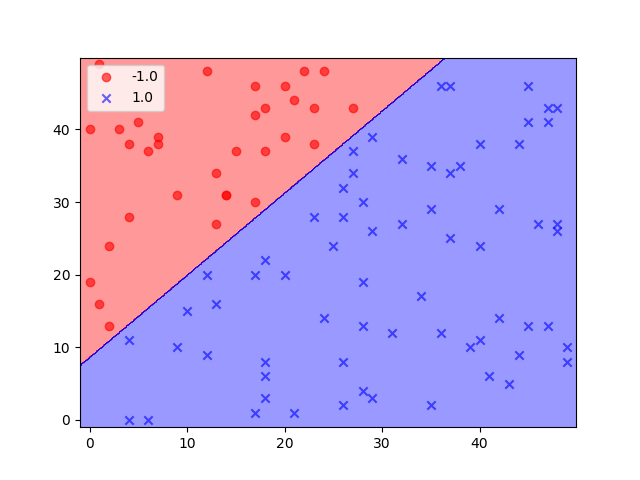
\includegraphics[width=15cm]{sample_linear.png}
\caption{sample\_linear.dat}
\end{figure}

\subsection{sample\_circle.dat}
sample\_circle.dat をGaussカーネル($\sigma$ = 10)SVMで学習すると図2がプロット結果として得られた。
\begin{figure}[!h]
\centering 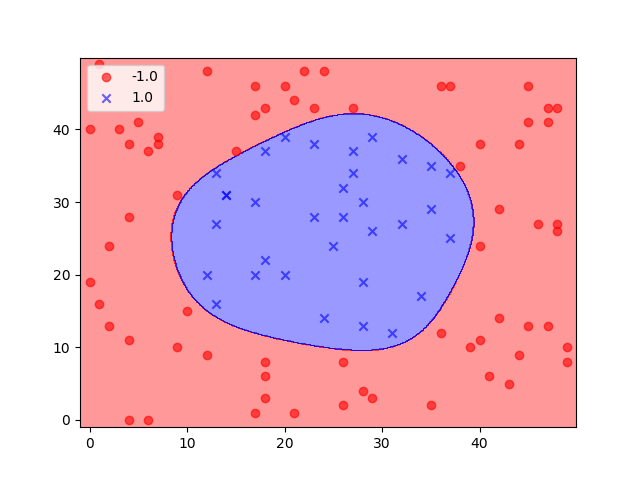
\includegraphics[width=15cm]{sample_circle.png}
\caption{sample\_linear.dat}
\end{figure}

\subsection{poly\_five.dat}
1次元データx=[1, 2, 5, 7, 8], y=[1, 1, -1, -1, 1]をpoly\_five.datとする。
このとき、$\alpha$について以下のような結果が得られた。
\begin{lstlisting}
alpha: 
0 [2.86101852e-09]
1 [1.01333335]
2 [8.47919771e-08]
3 [4.07999985]
4 [3.06666658]
\end{lstlisting}

\section{考察}
sample\_circle.datなど線形分離不可能なデータ点に対しては、線形SVMでは2次計画問題を解くことができずに
プログラムが終了した。一方、カーネルSVM(たとえばGauss)では、パラメータを適切に設定することで
データ点を高次元空間に射影して、非線形の決定境界でクラスを正確に分類することができた。
線形SVMで2次計画問題が解けずに終了するのではなく、ソフトマージンを実装してある程度の精度で分類できるように
したい。

SVClassifier.predict の実装について、はじめは
\begin{lstlisting}
def predict(self, tX):
    batch_size = tX.shape[0]
    preds = []
    for i in range(batch_size):
        res = 0
        for j in range(self.__n):
            res += self.__alpha[j] * self.__y[j] * self.__kf(self.__X[j], tX[i])
        res -= self.__theta
        preds.append(np.sign(res))
    return np.array(preds)
\end{lstlisting}
のように実装していたが、このとき"./main.py data/sample\_circle.dat g 10.0"(resolution=0.1)を実行すると
グラフを表示するまでに自分の環境では10分27秒必要だった。
これは、計算量を概算すると、この実装では batch\_size(予測するデータのサイズ) * n(訓練データのサイズ)の計算量であり、
x1, x2がおよそ(0, 50)の範囲で、0.1の幅でグリッド点を取ることを考えると、500*500*100と膨大になるためである。
kernel関数をバッチ入力に対応させて、訓練データのサイズ分のfor文を無くした実装に変更すると自分の環境で0分8秒で実行できる
ようになった。

\section{参考資料}
\begin{itemize}
    \item Python機械学習プログラミング Sebastian Raschka 著
    \item はじめてのパターン認識 平井 有三 著
\end{itemize}

\end{document}